\section{Design for Motivation}\label{sec:motivation}

Research in motivation is commonly divided into three areas:

\begin{itemize}
\item Self-determination - the student is driven by a genuine wish that comes from themselves
\item Achievement - the student is driven by extrinsic motivations, to be rewarded
\item Expectation value - the student is driven by extrinsic motivations, but it is not coming from being rewarded
\end{itemize}

\cite{koballa} and \cite{abell} provide an overview of theories developed for these three areas. Further, \cite{fulmer} provides a review of methods to collect data which can be used to study motivation. \cite{deci} and \cite{ryan} studies self-determination theory, \cite{elliot} studies achievement theory, and \cite{eccles} and \cite{wigfield} studies expectancy-value theory.

In terms of product development, \cite{sierra} argues that if you have designed for the user's compelling context the user is already motivated (by self-determination). Then, the motivation of the user is to become better (achieve). \cite{sierra} suggests the focus to be how to help users progress (see "Progress and payoffs", achieve), and what pulls them off (see "Cognitive load theory" below). See figure \ref{fig:sierra-summary}, for a summary of her focus on designing for building expertise.

In terms of using the product in a training environment, expectation value becomes relevant. Research within training transfer \citep{brinkerhoff} shows that before and after is as important as the training itself. To design for this, the leader should be involved with the participants before the training, and communicate expectations. The student should be expected to implement the training in everyday life \citep{brinkerhoff}. Both of these aspects holds true for the YoungDrive program, and how a teacher communicates the use of an app needs to be taken into consideration.

\begin{figure}[h]
  \centering
  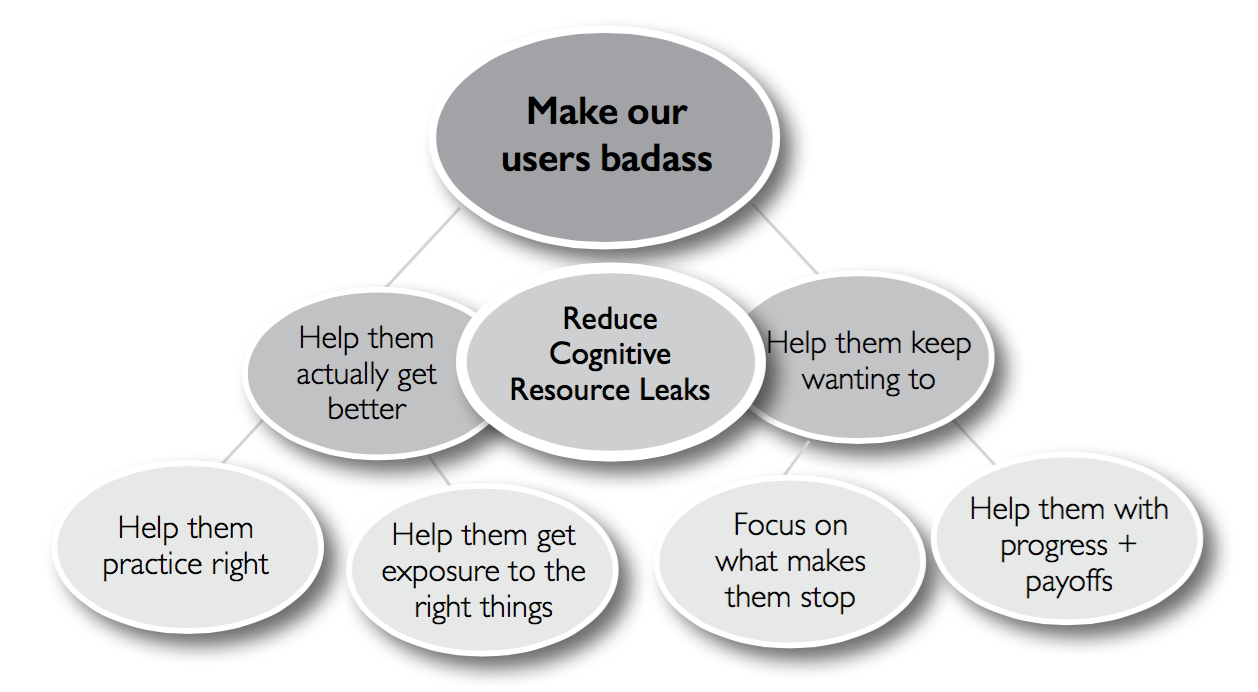
\includegraphics[width=0.8\textwidth]{SierraSummary.png}
  \caption{\cite{sierra} shares how to design for "making users awesome", meaning that a strategy for building an appreciated product is to help the user become good in something that appeals to her, i.e. to design for the compelling context. She then mentions barriers to not learning, like motivational aspects like reducing cognitive load and helping the user to progress.}
  \label{fig:sierra-summary}
\end{figure}

\subsection{Cognitive Load Theory}

\cite{sierra} argues that working on what stops people matters more than working on what entices them. Thus, a focus needs to be identifying and removing stumbling blocks. She then describes how humans have scarce cognitive resources, and how to design for these. Cognitive load theory (CLT) research is divided into three types of load: intrinsic load (stumbling blocks), extrinsic load, and germane load \citep{sweller}. Below, to design for these are described.

Intrinsic load needs to be dealt with if the effort to perform a task is too high. \cite{sierra} describes two strategies. She first says that according to deliberate practice, if you can not get to 95\% reliability within three 45-90 minute sessions, split skills that can be done with effort into sub-skills. The purpose is to reduce time spent practising being mediocre. Extraneous load, is about the way information is presented to a learner, and should be handled via designing to support cognitive resources, Sierra says \citep{sierra}. Germane load, is the work put into creating a permanent store of knowledge. To make the knowledge permanent, make sure the learner believes the information is essential, \cite{sierra} says: either by designing for the compelling context, or designing for just-in-time learning versus just-in-case.

Scaffolding is a technique to step by step remove the support wheels for the user, e.g. present information in different ways. \cite{gates} shows that in their research, each category of scaffolding demonstrated significant effects on learning. Another way to reduce cognitive leaks is don't make users memorise unnecessary things: make the thing you want the user to do, the most likely thing to do (accordances). Everything that takes willpower, reduces cognitive leaks.

The rule of thumb in applying cognitive load theory is that you want to decrease extraneous load, bad load, and increase germane load, good load. For example, in the case of a quiz app, the visual presentation of the questions can reduce extraneous load by removing unnecessary information. Germane load can be increased by giving scaffolding support at the end of each section, for example helping users to remember, by showing them their answers.

\subsection{Progress and Payoffs} \label{progress-payoffs}

\cite{sierra} argues that to pull users forward, to stay motivated, progress and payoffs are essential. Both of these, are investigated in terms of motivational psychology.

The feeling of progress can be emphasised by a path with guidelines to help the user know where they are at each step, e.g. for a training. To create a path, she encourages the designer to make a list of key skills ordered from beginner to expert. Then, these are sliced into groups of ranking or levels.

This way, it is possible to design a “belt” path for your context. The first level, should feel like a superpower for the user. The best payoff, is a intrinsically rewarding experiences, according to \cite{sierra}. For an entrepreneur, gaining the skills of selling (the progress) can be as rewarding as having gained the money for it (the payoff).

For motivation, the earlier, lower levels should be achievable in far less time and effort than the later, advanced levels. One practice is to try to have each new level take roughly double the time and effort of the previous level. This highly relates to flow.

Caring for the compelling context, why the user wants to learn the skill, are helpful strategies. A sometimes critiqued way of progression is to give the user high pay-off tips, but if done in a fair way, it is a good way for both learning and motivation.

This kind of path map is superb to simple gamification, says \cite{sierra}. In an app for building entrepreneurship coach skills, the act of becoming certified (getting 100\% correct), might not be as rewarding as the progress of getting there. Therefore, gamification of the sort "rewarding effort" might be more beneficial with "rewarding result". Suitable gamification could also mean unlocking new possibilities of adding value to the app (for example adding questions to the quiz), versus getting a badge or a star.

The shown benefits of designing for intrinsic motivation is in-line with self-determination theory \citep{deci, ryan}.  \cite{pink} concludes that the surprising truth about what motivates us is that drive is fostered by autonomy, mastery and purpose. Meanwhile, \cite{gates} says that simple gamification as well as more sophisticated game mechanics can prove effective. However, he adds that it should be investigated if "simple gamification" (e.g. contingent point and badges connected to learning activities) more frequently focus on lower-order learning outcomes, compared to studies with more sophisticated game mechanics. For the case of entrepreneurship, the goal is on higher-order learning outcomes, meaning simple gamification is not enough to motivate users. Thus, if you do not design for the compelling context, entrepreneurship coaches may well prefer other learning methods instead of using your gamified app.
